\section{System Development}

\subsection{UML Diagrams}

Some of the UML diagrams that we made for this system are given below.

\subsubsection{Use Case Diagram}

\begin{figure}[h!]\centering
  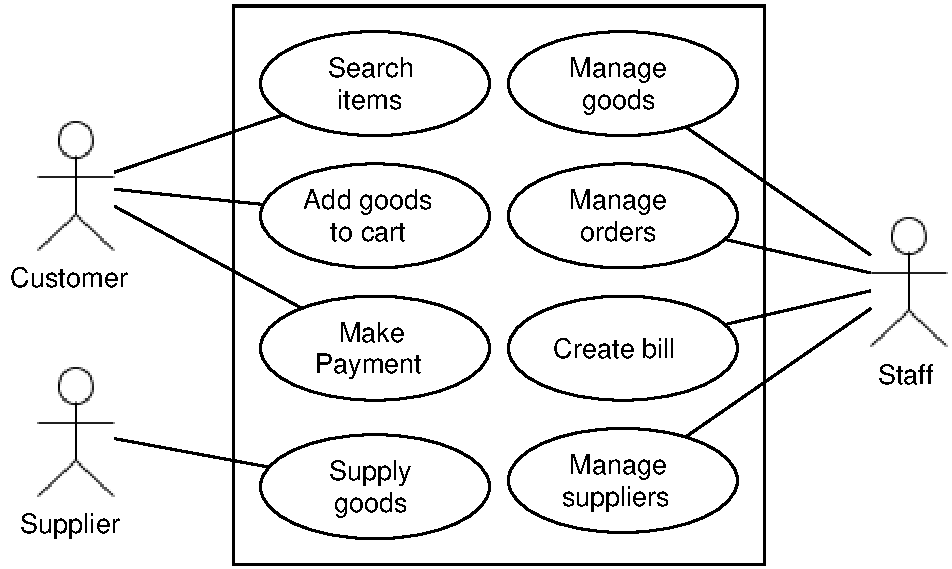
\includegraphics[width=4in]{fig/use-case}
  \caption{Use case diagram}\label{fig:use-case}
\end{figure}

\subsubsection{Class Diagram}

Class diagram is shown below. It mainly consists of different classes and their
relationship (association, generalization)

\begin{figure}[h!]\centering
  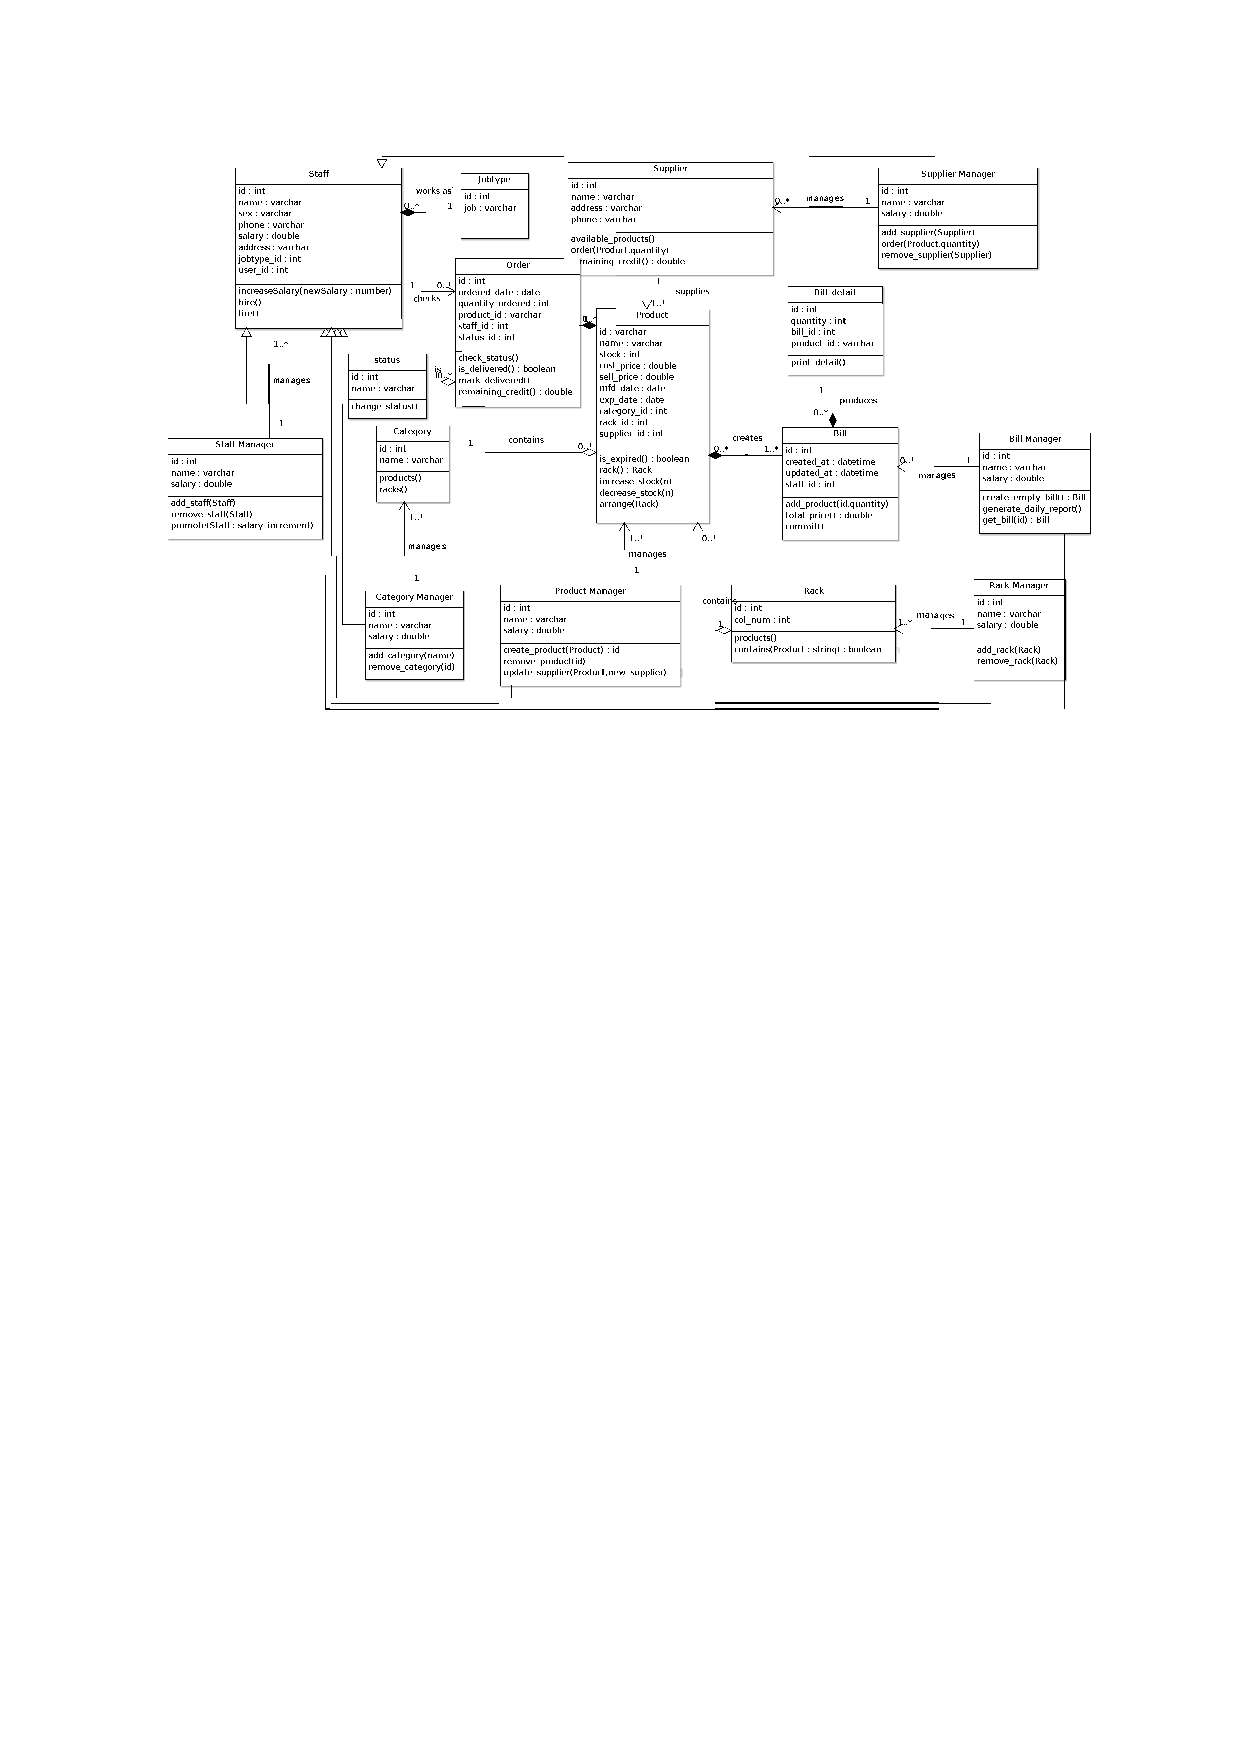
\includegraphics[width=\textwidth]{fig/class}
  \caption{Class diagram}\label{fig:class}
\end{figure}


\subsubsection{Sequence Diagram}

This diagram describes sequence of steps that may commonly occur in the
department store. We have five objects namely Department Store, Product,
Supplier, Customer, and Bill. Department Store checks for product status for
each product i.e. quantity (available stock), quality (exp date, condition
during storage), cost and updates the current status. Accordingly, it orders
goods/products from various suppliers and arrange them in store, Customers
come, search for product and buy required product. They find cost for each
product in label sticked to each product. A bill is made per transaction and
product is handed to customers after bill clearance. The activities like
searching product and buying product may happen several times (shown in diagram
explicitly as a loop). After the transaction is complete, store updates product
status and now has current status of the products.

\begin{figure}[h!]\centering
  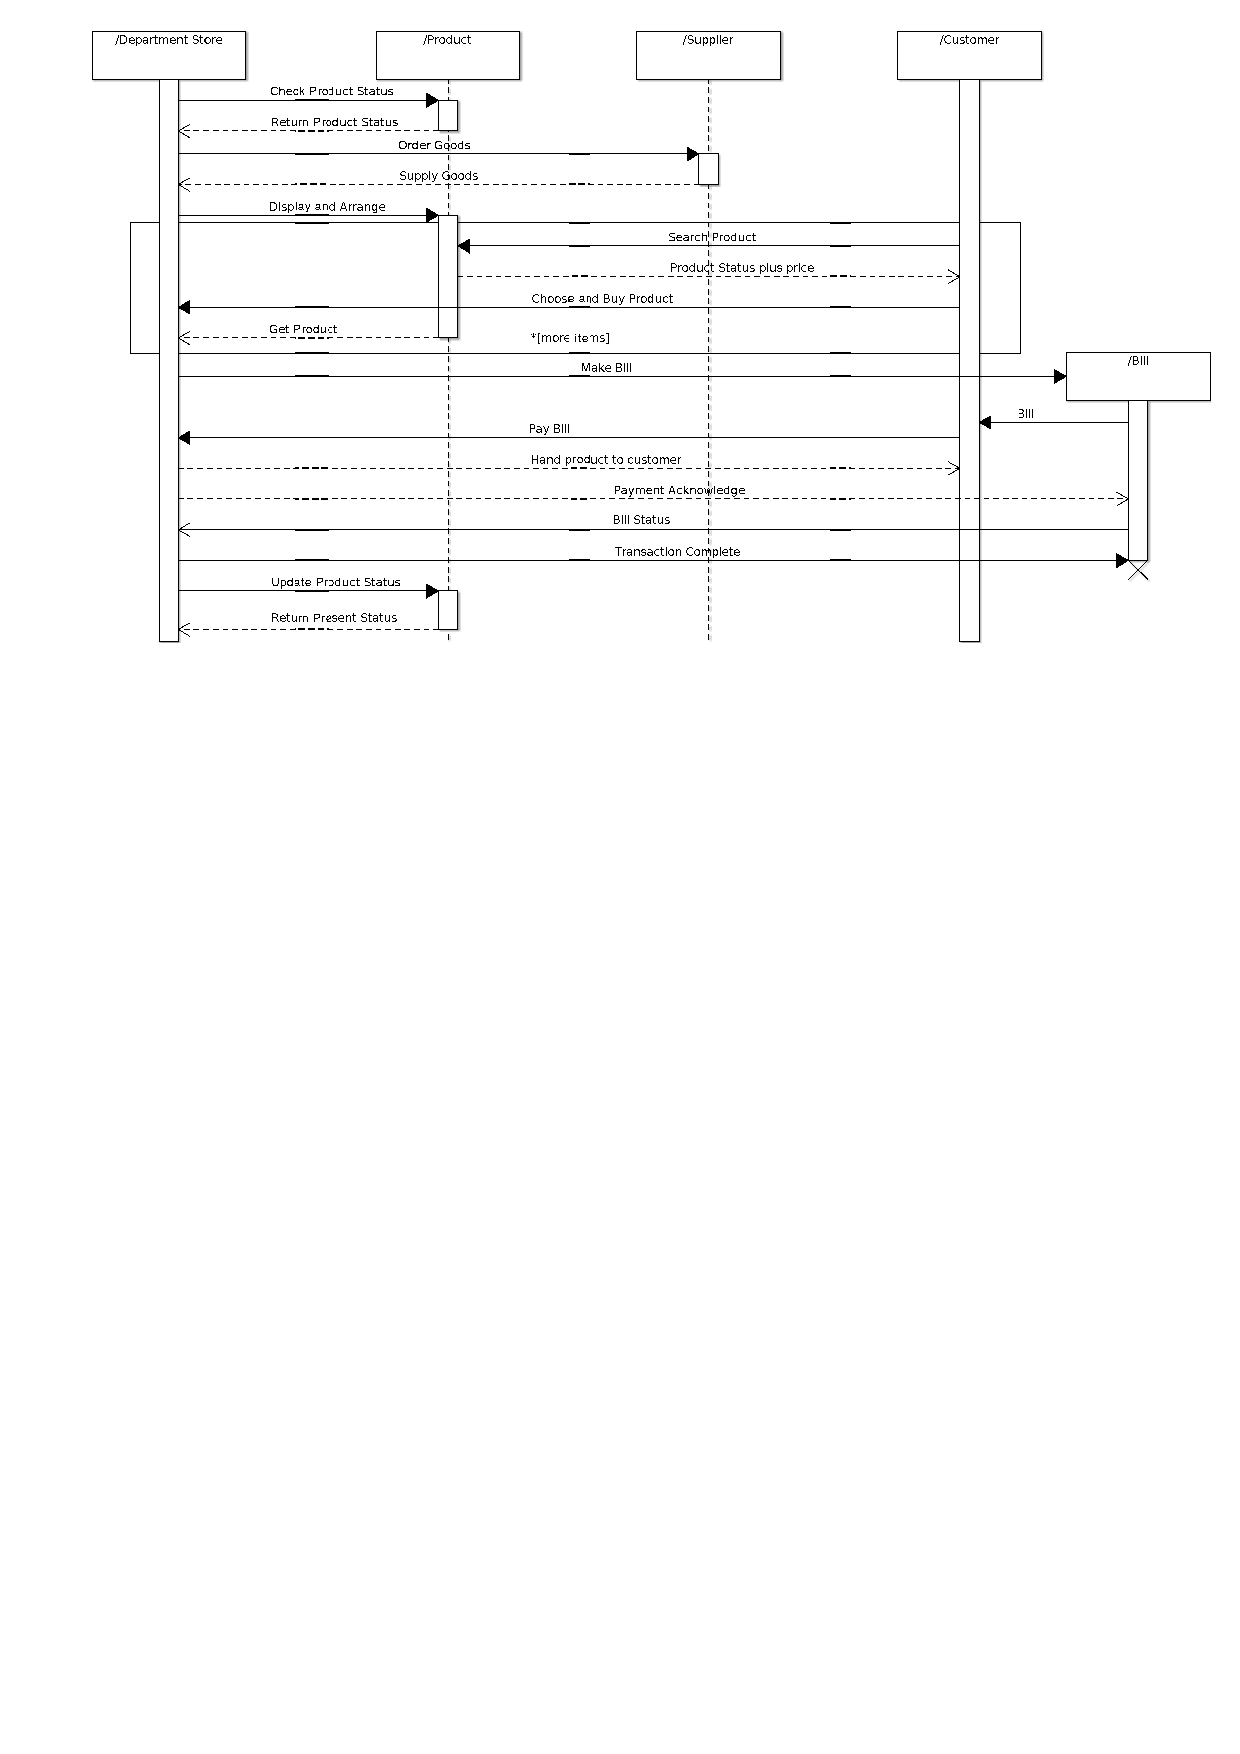
\includegraphics[width=\textwidth]{fig/sequence}
  \caption{Sequence diagram}\label{fig:sequence}
\end{figure}


\subsubsection{Activity Diagram}

This diagram shows user oriented view of system operation. There are states for
every work/operation that may happen in department store.

\begin{figure}[h!]\centering
  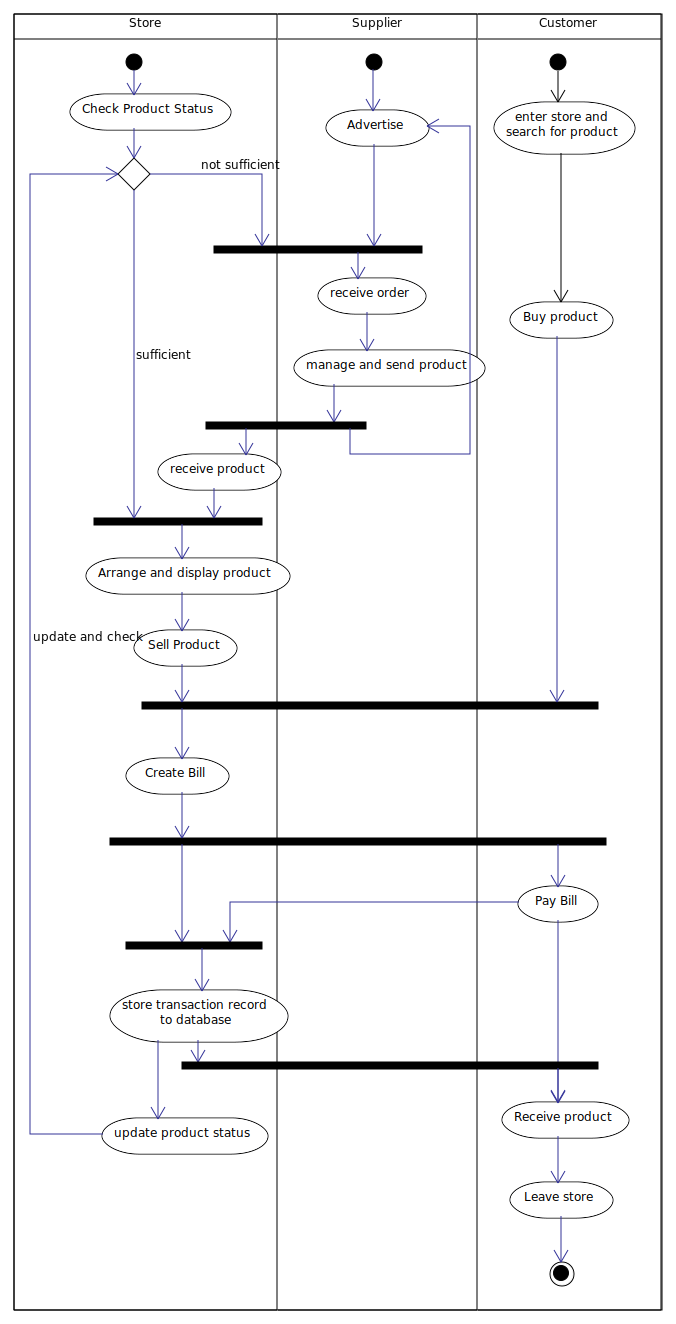
\includegraphics[height=\textheight-1cm]{fig/activity}
  \caption{Activity diagram}\label{fig:activity}
\end{figure}


\subsubsection{Collaboration Diagram}

Sequence diagram and collaboration diagram are very much similar to each other
that deals with instances and not classes. Collaboration diagram shows sequence
of steps needed for operation of system in graph-like structure. Sequence of
step is explicitly written before each operation association between instances.

\begin{figure}[h!]\centering
  \includegraphics[width=\textwidth]{fig/collaboration}
  \caption{Collaboration diagram}\label{fig:collaboration}
\end{figure}


\subsubsection{State Chart Diagram}

These diagrams depict the way in which objects evolve during their life in the
system. The elements of state chart diagram are:
\begin{description}
  \item[States] representing a stable condition of the object which persists
    for a significant time
  \item[Transitions] depicting possible paths from one state to another.
  \item[Events] these may be external events originating from actors, or
    internal events performed by other objects in the system.
  \item[Actions] processing carried out as part of a transition in state
  \item[Conditions] conditions governing the occurrence of a transition.
\end{description}

\begin{figure}[h!]\centering
  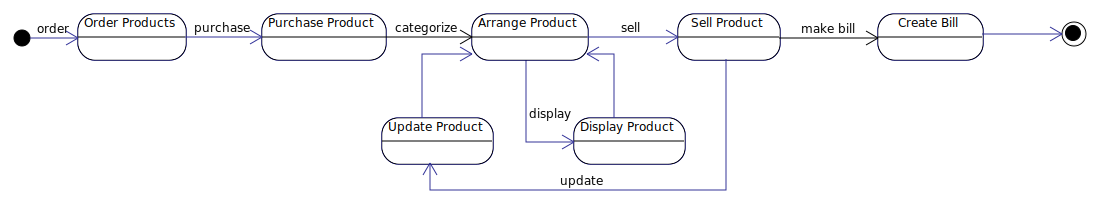
\includegraphics[width=\textwidth+1cm]{fig/state-chart}
  \caption{State chart diagram}\label{fig:state-chart}
\end{figure}


\subsection{Data Flow Diagrams}

\subsection{Entity Relationship Diagrams}

\begin{figure}[h!]\centering
  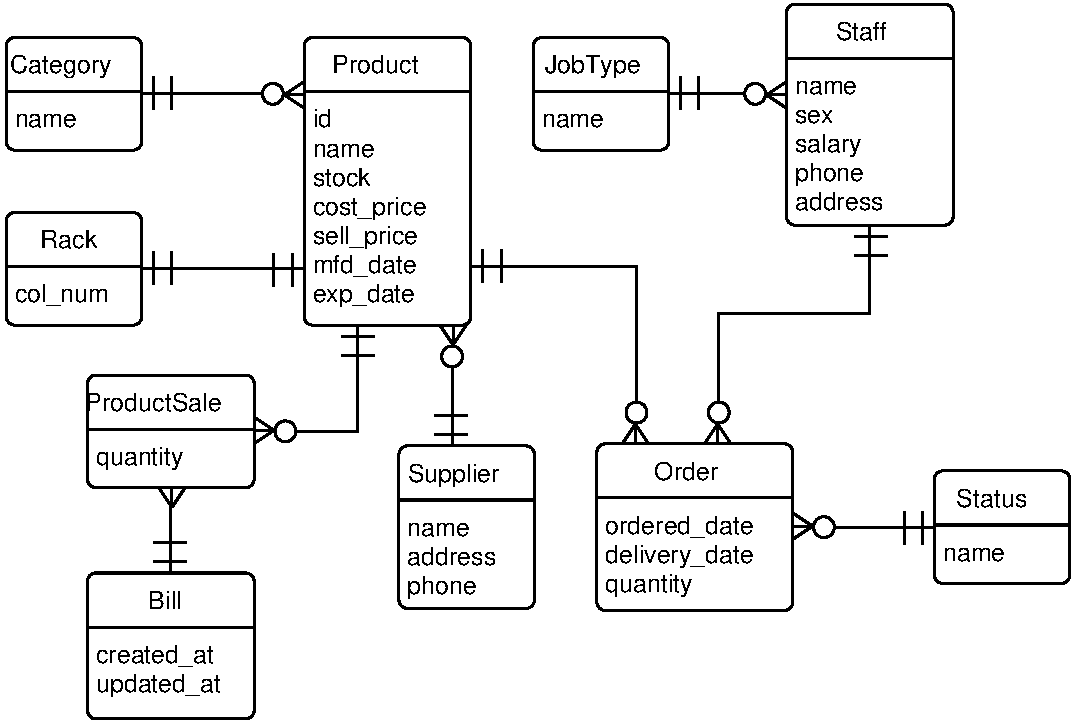
\includegraphics[width=\textwidth]{fig/erd}
  \caption{Entity relationship diagram}\label{fig:erd}
\end{figure}
